\documentclass[11pt,a4paper,oneside]{article}
\usepackage[utf8]{inputenc}
\usepackage[french]{babel}
\usepackage[T1]{fontenc}
\usepackage{graphicx}
\usepackage{charter}
\usepackage{hyperref}
\usepackage{listings}
\usepackage[left=2cm,right=2cm,top=2cm,bottom=2cm]{geometry}
\author{Mylann Dupuy}
\title{Dossier de Solution}
\date{10 Mars 2017 -- Version 3}
\begin{document}
\maketitle
\begin{figure}[hbtp]
\centering

\includegraphics[scale=1]{Script/cjb.jpg}
\end{figure}
\newpage
\tableofcontents
\newpage
\setcounter{page}{3}
\section{Contexte}
Le centre Jean Bernard / Clinique Victor Hugo voudrait mettre un nouveau système de déploiement pour installer et/ou mettre à jour les logiciels existants.

\section{Objectif(s)}
L'objectif est de déployer les logiciels utilisés couramment et de les mettre à jour sous Windows Server ou sous Linux Server. Le système doit fonctionner en faisant l'inventaire sur les 3 Sites (Le Mans - Chartres - Caen). 

\subsection{Cahier des charges}
Il faut déployer l'ensemble des Postes sur les réseaux du Centre Jean Bernard - Clinique Victor Hugo sans que cela dérange les utilisateurs, il faut donc mettre en place un système de déploiement pour mettre à jour ou installer des logiciels manquants sur les Postes.\\ \\
\textbf{Voici les logiciels à déployer :}\\

\begin{itemize}
	\item Adobe Flash Player 24
	\item Adobe Reader DC
	\item Java 8 Update xx
	\item Mozilla Firefox
	\item Mozilla Thunderbird
	\item PDFCreator
	\item TightVNC
	\item 7-Zip
\end{itemize}

\begin{center}
\textbf{Tous les logiciels doivent être installés avec des paramètres spécifiques !}
\end{center}
\subsection{Contraintes}
Lors du déploiement, les Postes sont constamment utiliser par le personnel du centre. Pour pouvoir intervenir, il faut appeler la personne présente sur le poste et intervenir à distance avec \textbf{TightVNC}.\\

Tous les Postes n'ont pas la même fonction donc il faut mettre à jour les logiciels déjà présents.

\subsection{Matériels disponibles}
\begin{itemize}
	\item \textbf{1 Ordinateur} pour administrer l'un des serveurs via SSH.
	\item \textbf{1 Serveur virtuel} sous \textbf{Debian 8.7} ou \textbf{Windows Server 201x}.
	\item \textbf{1 Serveur de stockage} pour l'accès aux exécutables prévus pour les scripts. 
\end{itemize}
\newpage

\section{Solutions}
\subsection{Comparaison}
En cherchant sur Internet et aussi avec nos connaissances personnelles, 4 solutions de déploiement ont été recensées.\\ \\
%%%%%%%%%%%%%%%%%%%%%%%%%%%%%%%%%%%%%%%%%%%%%%%%%%%%%%%%%%%%%%%%%%%%%%%%%%%%%%%%%%%%%%%%%%%%%%%%%%%%%%%%%%%%%%%
\begin{tabular}{|p{3.1cm}|p{6.5cm}|p{6.5cm}|}
	\hline
	\centering Solutions : & \centering Avantages : & Inconvénients : \\
	\hline
	%%%%%%%%%%%%%%%%%%%%%%%%%%%%%%%%%%%%%%%%%%%%%%%%%%%%%%%%%%%%%%%%%%%%%%%%%%%%%%%%%%%%%%%%%%%%%%%%%%%%%%%%%%%
	\centering OCS Inventory NG  & \begin{itemize}
							\item Faible utilisation de la bande passante 
							\item Plugins pour GLPI							
							\item Supervision des logiciels installés
							\item Logiciel libre disponible sous Windows Server/Client ou Linux Server/Client
							\item Inventaire complet des Postes							
									\end{itemize} & \begin{itemize}
												\item Wiki non à jour  
												\item Paquets Debian en version 2.0.5
										\end{itemize} \\
	\hline
	%%%%%%%%%%%%%%%%%%%%%%%%%%%%%%%%%%%%%%%%%%%%%%%%%%%%%%%%%%%%%%%%%%%%%%%%%%%%%%%%%%%%%%%%%%%%%%%%%%%%%%%%%%%
	\centering WAPT  & \begin{itemize}
							\item Automatisation d'installation, MAJ et suppressions logiciels 
							\item Centralisation graphique du déploiement
							\item Facilité pour les MAJ 
							\item Gestion des dépendances
							\item Logiciel libre													
						\end{itemize} & \begin{itemize}
												\item Configuration à faire pour faire cohabiter WSUS et WAPT 
												\item Packages propres à WAPT (.wapt)
												\item Suite Microsoft Office non disponible
												\item Création de paquets + ou - complexe
												\item Certains logiciels ne sont plus à jour			
										\end{itemize} \\
	\hline
		%%%%%%%%%%%%%%%%%%%%%%%%%%%%%%%%%%%%%%%%%%%%%%%%%%%%%%%%%%%%%%%%%%%%%%%%%%%%%%%%%%%%%%%%%%%%%%%%%%%%%%%%%%%
	\centering WSUS Package Publisher  & \begin{itemize}
							\item Utilise les packages .EXE et .MSI 
							\item Cohabite avec WSUS en reprenant toute la BDD WSUS					
							\item Déploiement des packages
							\item Génère un certificat auto-signé en utilisant une GPO configurée
									\end{itemize} & \begin{itemize}
												\item  Si le WSUS est en panne, le déploiement n'est plus possible									
										\end{itemize} \\
	\hline
	%%%%%%%%%%%%%%%%%%%%%%%%%%%%%%%%%%%%%%%%%%%%%%%%%%%%%%%%%%%%%%%%%%%%%%%%%%%%%%%%%%%%%%%%%%%%%%%%%%%%%%%%%%%
	\centering GPO  & \begin{itemize}
							\item Facile d'installation des paquets MSI
																			
						\end{itemize} & \begin{itemize}
												\item Ralentis l'ouverture de session
												\item Installe que les Packages .MSI	
										\end{itemize} \\
	\hline
\end{tabular}
%%%%%%%%%%%%%%%%%%%%%%%%%%%%%%%%%%%%%%%%%%%%%%%%%%%%%%%%%%%%%%%%%%%%%%%%%%%%%%%%%%%%%%%%%%%%%%%%%%%%%%%%%%%%%%
\\ \\
Nous avons décidé de mettre en place \textbf{OCS Inventory NG 2.3} (cf.Références) car les logiciels qui doivent être déployé seront facilement mis à jour contrairement à WAPT qui à certains logiciels non à jour voir même abandonner.
\newpage
\subsection{Mise en \oe{}uvre}
\subsubsection{Avant de commencer} 
Nous avons créé une machine virtuelle sous Hyper-V (cf.Références) en lui mettant comme ressources :\\ \begin{itemize}
				\item 1 image ISO de Debian 8.7
				\item 4 Go de mémoire vive
				\item 1 C{\oe}ur dédié
				\item 50 Go d'espace disque
				\item 1 connexion au réseau CJB	
\end{itemize} 

\begin{center}
\textbf{Cette configuration est hébergée virtuellement}
\end{center}
\subsubsection{Installation}
Lors de l'installation, il faut tout laisser par défaut sauf le proxy qui doit être renseigné. Suite à l'installation, il reste à installer \textbf{openssh-server} pour tout faire via \textbf{PuTTY} ou \textbf{SSH} .\\

Depuis PuTTY ou SSH, il faut installer le serveur Web, le serveur BDD, PHP, Perl et leurs modules (\textbf{apache2, mylsql-server, php5, perl, libxml-simple-perl, libcompress-zlib-perl, libdbi-perl libdbd-mysql-perl,libapache-dbi-perl, libnet-ip-perl, libsoap-lite-perl}).\\ \\
Pour les modules Perl en cas de problèmes de paquets, il faut les télécharger et les installer à la main depuis ce site \url{http://search.cpan.org/} 
S'il manque des paquets, le script d'installation d'OCS Inventory les installera, mais dans notre cas, on est derrière un proxy, mais il est préférable de tout installer avant. \\

Pour installer OCS Inventory NG, il faut utiliser l'archive qui était sur le site et la documentation qui n'est pas à jour (cf.Références).
\newpage
\section{Déploiement}
\subsection{Principe de fonctionnement}
\begin{figure}[hbtp]
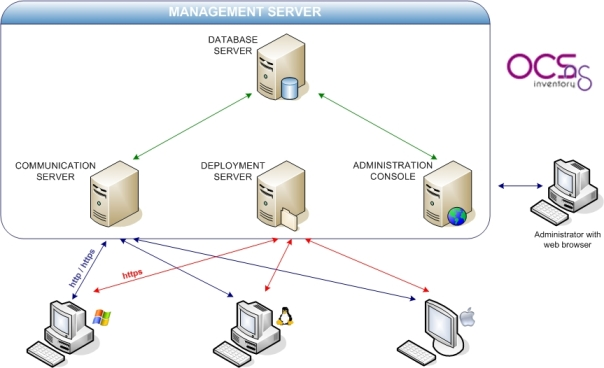
\includegraphics[scale=0.8]{Script/deploy.jpg}
\caption{Schéma de déploiement (Source : Wiki OCS)}
\end{figure}
L'architecture reste simple à mettre en place, dans l'environnement actuel nous avons tout mis sur le même serveur.
\subsection{Outil de déploiement}
\subsubsection{OCS Inventory NG Agent Deployment Tool}
\begin{figure}[hbtp]
\centering
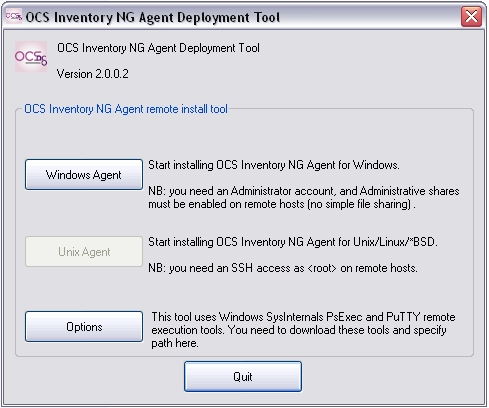
\includegraphics[scale=0.5]{Script/1.jpg}
\caption{Etape 1 - Écran de démarrage}
\end{figure}
Avant de faire le déploiement de logiciels sur le réseau, il faut installer l'agent OCS sur les Postes Clients avec \textbf{OCS Inventory NG Agent Deployment Tool} puis aussi vérifier si les partages administratifs (C\$) sont bien activés. Pour ce faire, il faut faire \textbackslash\textbackslash 192.168.x.x\textbackslash C\$
 puis passer à \textbf{l'étape 2}. Si ça ne fonctionne pas, allez dans le Pare-Feu et autorisez le \textbf{"Partage de Fichiers et d'imprimante"}.
\newpage

\begin{figure}[hbtp]
  \centering
  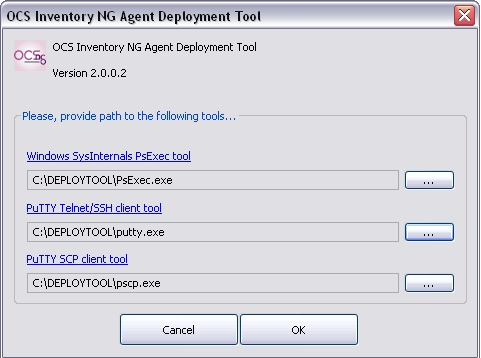
\includegraphics[scale=0.5]{Script/2.jpg}
  \caption{Etape 2 - La configuration de l'outil de déploiement}
\end{figure} 
Dans notre cas, il faut déployer l'agent sur les Postes Clients mais pour ce faire, il faut utiliser le module \textbf{PSEXEC} (cf.Annexes) depuis le poste qui va déployer l'agent OCS. Il suffit de mettre le répertoire exact du module précédemment téléchargé depuis le site dans les options d'OCS Inventory NG Agent Deployment Tool. Quand c'est fait, il faut passer à \textbf{l'étape 3}. \\

\begin{figure}[hbtp]
 \centering
 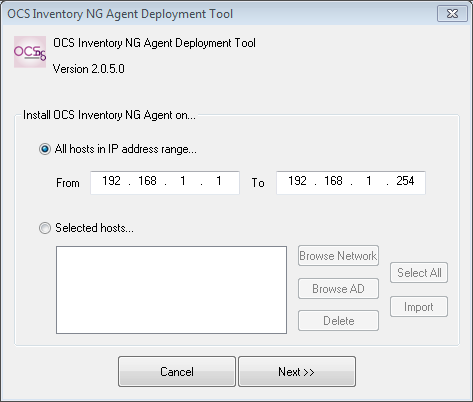
\includegraphics[scale=0.7]{Script/3.png}
 \caption{Etape 3 - La sélection des Postes}
 \end{figure}
  
\textbf{L'étape 3} consiste à définir une plage IP  ou à sélectionner le(s) Poste(s) qui auront l'agent OCS. Dans notre cas, on avait défini une plage IP sur l'ensemble du réseau CJB. Après la sélection des Postes, on passe à \textbf{l'étape 4}.
\newpage

\begin{figure}[hbtp]
\centering
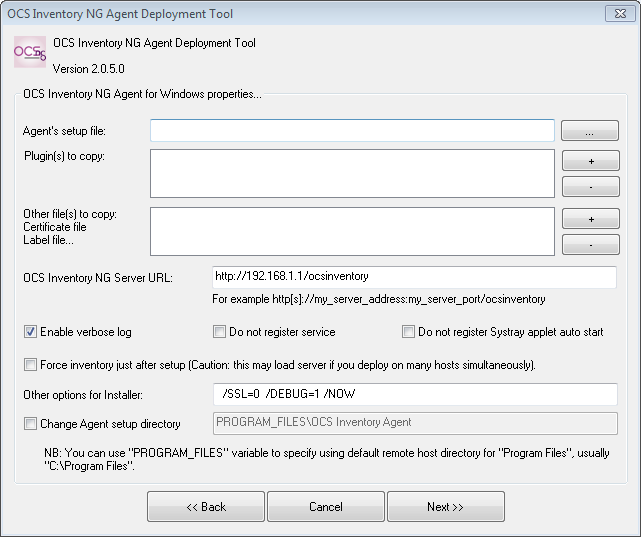
\includegraphics[scale=0.7]{Script/4.png}
\caption{Etape 4 - Les paramètres de l'agent OCS}
\end{figure}

À partir de là qu'on va faire la configuration de l'agent OCS qui sera mis en place lors du déploiement.  
\begin{enumerate}
\item Il faut lui donner le répertoire où se trouve le fichier d'installation de l'agent sur le poste Administrateur.
\item Le(s) plugin(s) ou fichier(s) à copier sur le Poste Client.
\item Le certificat du serveur si SSL est activé sur le serveur OCS.
\item L'adresse URL du serveur OCS.
\item Activer les options pour l'agent OCS (Logs, Ne pas enregistrer en tant que service, Ne pas mettre l'icône dans la barre de notifications au démarrage du Poste, forcer l'inventaire après l'installation).
\item Les options spécifiques qu'on veut mettre. Les options choisies au-dessus sont écrites dans cet encadrement.
\item Le répertoire d'installation pour l'agent OCS sur le(s) Poste(s) Client(s).
\end{enumerate}
Quand cette étape est faite, on passe à \textbf{l'étape 5} qui terminera les étapes de configuration de l'agent.
\newpage
\begin{figure}[hbtp]
\centering
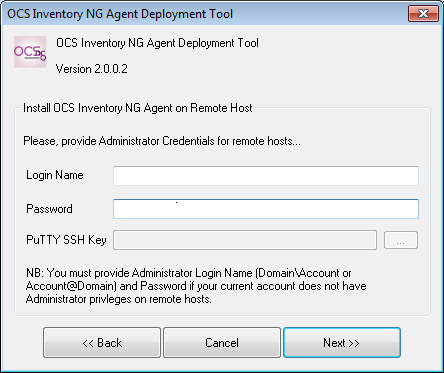
\includegraphics[scale=0.9]{Script/5.png}
\caption{Etape 5 - L'authentification}
\end{figure}

Pour permettre le déploiement de l'agent OCS SANS déranger les utilisateurs ni en intervenant sur les Postes Clients, il faut renseigner les informations de connexion du compte "Administrateur" du domaine pour les \textbf{Postes WINDOWS}. Si les informations sont exactes, on lance le déploiement à l'étape 6.

\begin{figure}[hbtp]
\centering
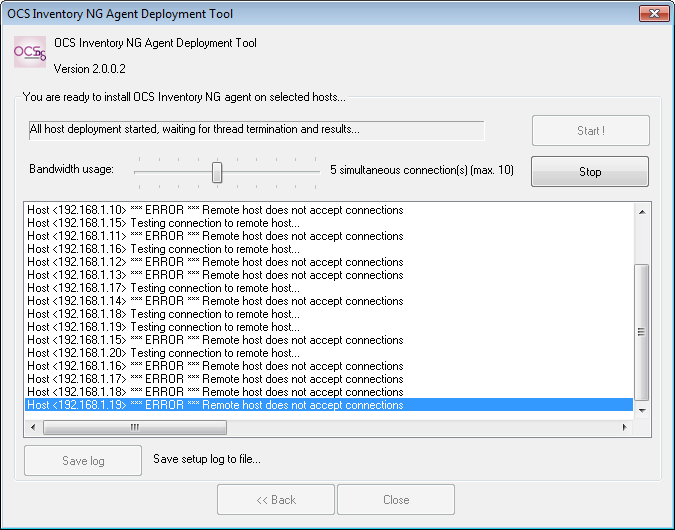
\includegraphics[scale=0.6]{Script/6.png}
\caption{Etape 6 - Log de déploiement}
\end{figure}

Suite à cette configuration, il suffit de lancer le déploiement pour installer et exécuter l'agent OCS sur les Postes Clients. L'outil de déploiement peut déployer les Postes Clients 1 par 1 ou peut faire 10 connexions simultanées, c'est-à-dire qu'il va faire l'opération sur 10 Postes maximum. \\ 
\textbf{ATTENTION ! En changeant le nombre de connexion simultanée, on augmente la charge du CPU du poste Administrateur.}
\newpage
\subsubsection{Via GPO}
Le déploiement de l'agent OCS consiste à l'installer automatiquement sur les postes clients dès que l'utilisateur va se connecter avec son \textbf{login//P@ssword} de l'AD. Suite à ça, l'agent va se déployer via un script mis au c\oe{}ur de la GPO du Windows Server 2012.
\\
\begin{figure}[hbtp]
\centering
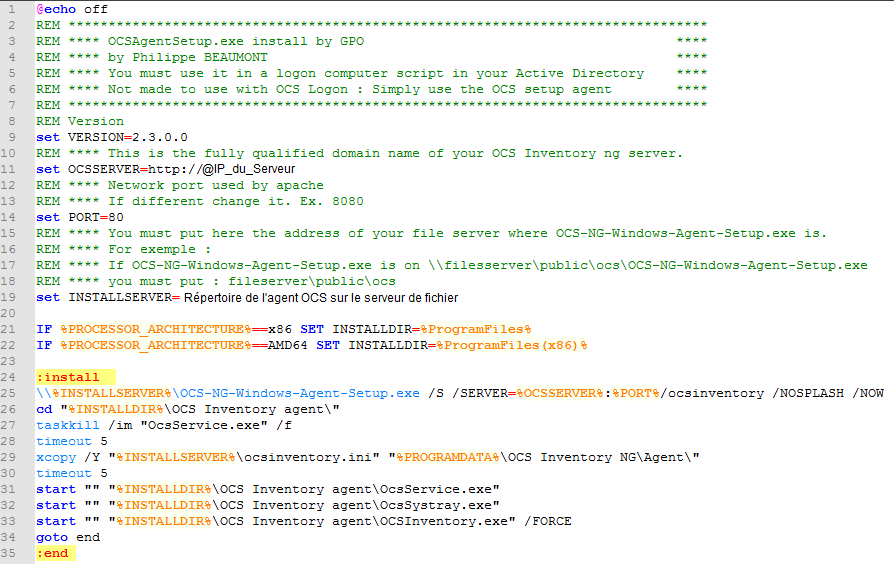
\includegraphics[scale=0.7]{Script/DeploiementGPO1.PNG}
\caption{Script de déploiement}
\end{figure}

Pour commencer, il faut faire le script qu'il faudra mettre sur l'Active Directory (\textbf{script inspiré de Philippe BEAUMONT}.\\
En détail : 
\begin{itemize}
\item Ligne 9 : La version de l'agent OCS
\item Ligne 11 - Ligne 14 : L'adresse IP et le port d'écoute du Serveur OCSInventory
\item Ligne 19 : Le répertoire où se situe le programme d'installation de l'agent qui sera déployé et qu'on inclut dans la variable "INSTALLSERVER"
\item Ligne 21 - Ligne 22 : Le répertoire d'installation sur les Postes Distants présents dans la variable "INSTALLDIR"
\item Ligne 25 : On exécute le programme d'installation en utilisant les variables et en rajoutant les options d'installation en spécifiant le serveur OCS par la variable, en installation silencieuse et en forçant l'inventaire après l'installation.
Ligne 27 - Ligne 30 : On "tue" le processus "OCSService" pour copier le fichier de configuration "ocsinventory.ini" dans le dossier de l'agent situé dans "\%PROGRAMDATA\%"
\item Ligne 31 - Ligne 33 : On exécute "OcsService.exe", "OcsSystray.exe" pour qu'il soit vu dans la barre de notification et on relance de "force" un inventaire avec "OcsInventory.exe" \\
\end{itemize}
Après que le script soit créé et mis sur le serveur, il reste à paramétrer la GPO en mettant le script dans \textbf{"Configuration ordinateur\textbackslash Stratégies\textbackslash  Paramètres Windows\textbackslash  Scripts (démarrage/arrêt)\textbackslash Démarrage"}
\newpage
\subsection{Interface Web OCS Inventory}
Lors que l'agent est bien installé sur les Postes Clients, l'agent va faire l'inventaire complet du poste et envoyer automatiquement l'inventaire au serveur. On pourra se faire une idée sur les logiciels qu'on doit déployer ou non. \\

En arrivant sur l'écran d'inventaire, on remarque les différentes informations sur les Postes Clients (TAG, Dernier Inventaire, Nom de l'ordinateur, L'utilisateur actuel, OS, Fréquences RAM / CPU) qui sont automatiquement inventoriés selon la configuration faite depuis le serveur.
\subsection{Scripts}

OCS Inventory peut déployer des paquets SEULEMENT s'ils sont en ".zip" ou ".tar.gz" donc avant de déployer un paquet, on va créer un script qui va lancer les installations des logiciels de manière silencieuse et avec des paramètres spécifiques.
\\ \\
Ce sont des scripts Batch qui ont été réalisés pour CHACUN des logiciels. Le contenu est quasiment le même sauf pour la désinstallation et l'installation qui demandent des options spécifiques (No reboot, silencieux, aucune interaction avec l'utilisateur).
\\ \\
Lors de l'installation des logiciels, il ne faut pas que cela perturbe le travail de l'utilisateur donc il ne faut AUCUNE interaction donc pas de boîte de dialogue ni d'autorisation utilisateur ni de "Pop-Up" et SURTOUT PAS de redémarrage surtout dans ce contexte.
\newpage
\textbf{On va prendre l'exemple de Mozilla Firefox avec le code disponible : (Définitions en Annexes)}
\\
\begin{figure}[hbtp]
 \centering
 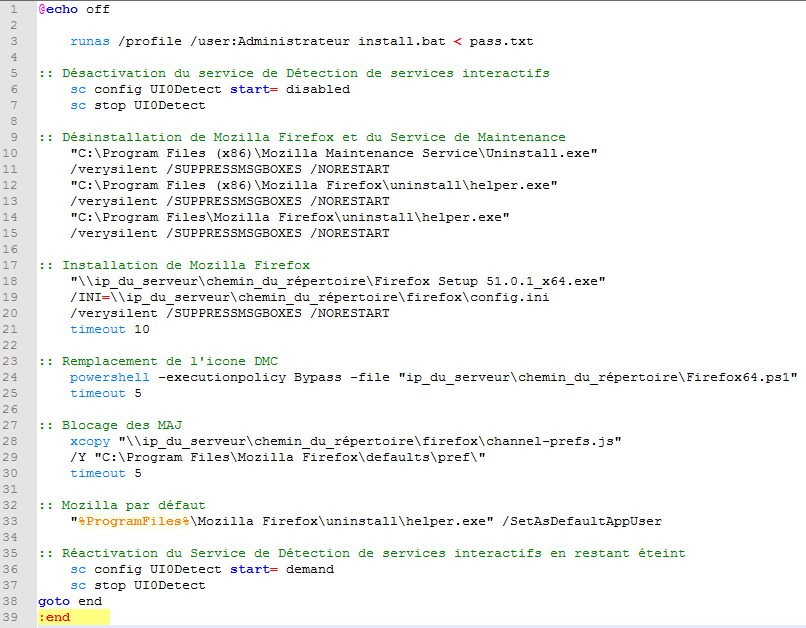
\includegraphics[scale=0.84]{Script/Firefox_annexes.PNG}
 \end{figure}  
\begin{itemize}
	\item Ligne 3 : Avec la commande \textbf{RUNAS}, on se connecte en tant qu'Administrateur sans charger le profil utilisateur, juste à avoir le privilège lors de l'exécution de ce script et pour pas à avoir à taper le mot de passe, le script utilise le fichier "pass.txt" qui contient le mot de passe en clair.
	\item Ligne 5 - 7: Il faut désactiver le service \textbf{U10Detect} (cf.Annexes) pour que rien n'apparaisse à l'écran. 
	\item Ligne 9 - 15 : Répertoire où se trouve le programme de désinstallation de \textbf{Mozilla Firefox} et de \textbf{Mozilla Maintenance Service}.
	\item Ligne 17 - 21 : Répertoire où se trouve le programme d'installation de \textbf{Mozilla Firefox} en utilisant son fichier de configuration (Répertoire d'installation du Poste Client, mettre ou non raccourcis sur le bureau ou la barre de lancement ou dans le menu démarrer, la désactivation du Maintenance Service). Faire l'installation silencieuse, supprimer tous les messages qui peuvent apparaître et ne pas redémarrer.
	\item Ligne 25 - 25 : Récupérer une icône, car l'ancienne ne fonctionnera plus (Cf.Problèmes rencontrés) en utilisant un script fait en \textbf{PowerShell}.
	\item Ligne 27 - 30 : Changement du canal de mise à jour de \textbf{Mozilla Firefox} pour pas qu'il puisse les faire.
	\item Ligne 32 - 33 : Faire de \textbf{Mozilla Firefox} le navigateur par défaut avec le paramètre
	\item Ligne 35 - 37 : Réactivation du Service de Détection de services interactifs en restant éteint
\end{itemize}
\newpage
\subsection{Phases de Tests}
À chaque fois qu'un script est fait ou modifié, le script est testé en local puis sur un poste de test.\\
\begin{itemize} 
	\item Est-ce que les \textbf{droits "administrateur"} sont bien mis ? Sinon, vérifier si le mot de passe est bon. 
	\item Est-ce que le script désactive le \textbf{service "U10Detect"} ? Sinon, vérifier si le service existe ou s'il est bien écrit dans le script
	\item Est-ce que le script \textbf{désinstalle le programme} ? Sinon, vérifier le répertoire où se trouve le programme de désinstallation.
	\item Est-ce que le \textbf{programme d'installation} s'est bien exécuté en installant le programme ? Si non, essayer d'accéder au serveur de fichiers.
	\item Est-ce que le \textbf{script} s'est déroulé de \textbf{manière "silencieuse"} ? Sinon, voir la syntaxe spécifique d'un fichier .EXE ou d'un Package .MSI. \\
\end{itemize}
Il faut regardé le fichier de log d'OCS dans "\textbf{\%PROGRAMDATA\%\textbackslash OCS Inventory NG \textbackslash Agent}" avec Notepad ou Notepad++ ou de voir dans \textbf{l'observateur d'événements}
\newpage
\subsection{Déploiement(s)}
\subsubsection{Création}
Il reste à créer l'archive en ".zip" avec le fichier ".txt" qui contient le mot de passe et le script Batch. En général, l'archive fait moins de 5 Kilo-Octets. Quand l'archive à bien été faite, il faut créer la fiche du déploiement en se connectant sur l'interface Web d'OCS et aller dans "Deployment" puis "Build"
\\
\begin{figure}[hbtp]
\centering
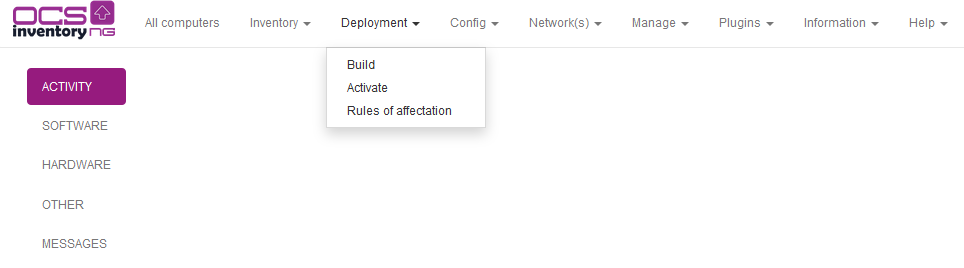
\includegraphics[scale=0.7]{Script/Deploiement1.PNG}
\caption{Accès Creation Déploiement}
\end{figure}
Après avoir cliqué dessus, la page \textbf{"Package Builder"} s'ouvre en y montrant un liste à remplir

Il faut renseigner \textbf{le nom}, \textbf{la description du paquet}, sur quel \textbf{OS} faut l'installer, \textbf{le protocole} (dans mon cas, j'ai pas mis en HTTPS), \textbf{la priorité} du déploiement (Chiffre le + haut est prioritaire), \textbf{le fichier} à déployer (mettre l'archive précédemment crée), \textbf{exécuter ou non} une commande à l'extraction du package donc la c'est le nom du script Batch. Le reste n'est pas à renseigner car on n'a pas de serveur de redistribution et on veut pas que l'utilisateur soit averti.
\begin{figure}[hbtp]
\centering
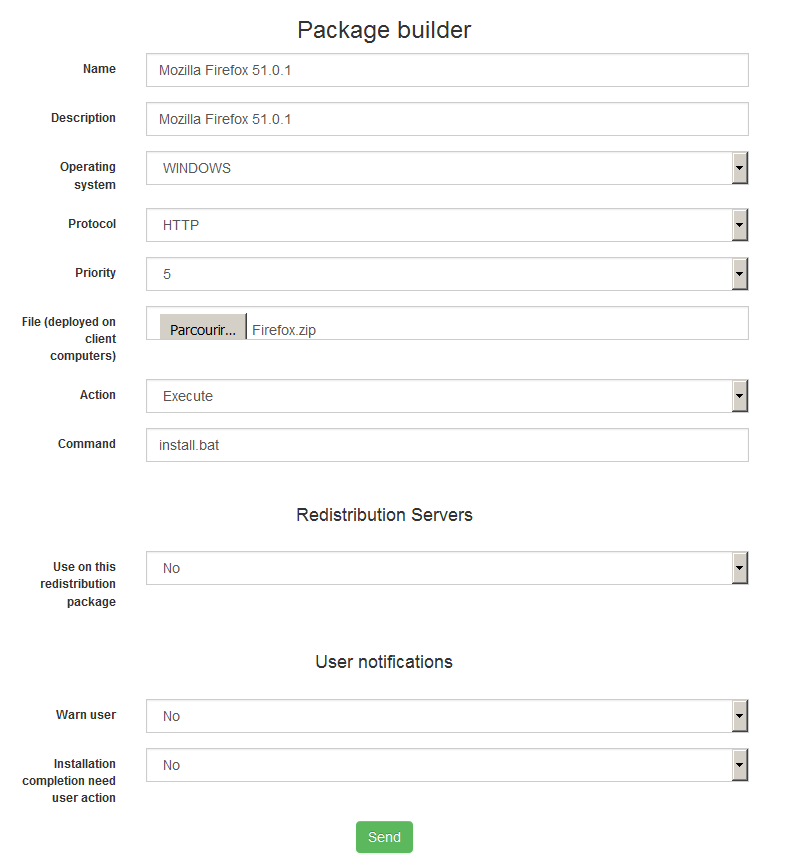
\includegraphics[scale=0.4]{Script/Deploiement2.PNG}
\caption{Information Déploiement}
\end{figure}

La page finale de création du paquet montre le \textbf{poids du paquet}, \textbf{le nombre} de fragment du paquets pour pas saturer le réseau lors du déploiement de gros paquet (ce n'est pas notre cas) et \textbf{le temps} estimé pour le déploiement (qui affiche souvent rien ou le mauvais temps)

\begin{figure}[hbtp]
\centering
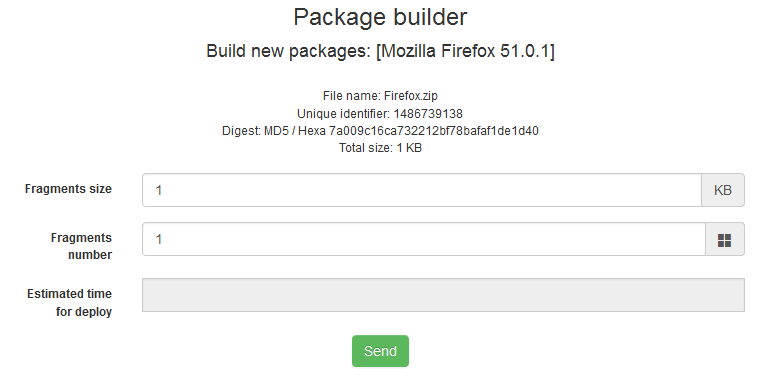
\includegraphics[scale=0.6]{Script/Deploiement3.PNG}
\caption{Résumé de création}
\end{figure}
\newpage
Dès que la confirmation apparait, cela veut dire que le paquets est bien créer dans le répertoire "/var/lib/OCSinventory-reports/download/......". On peut voir que tous les paquets de déploiement crées appartienne à "www-data"

\begin{figure}[hbtp]
\centering
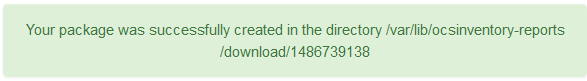
\includegraphics[scale=0.6]{Script/Deploiement4.PNG}
\caption{Confirmation de Création du paquets}
\end{figure}

\begin{figure}[hbtp]
\centering
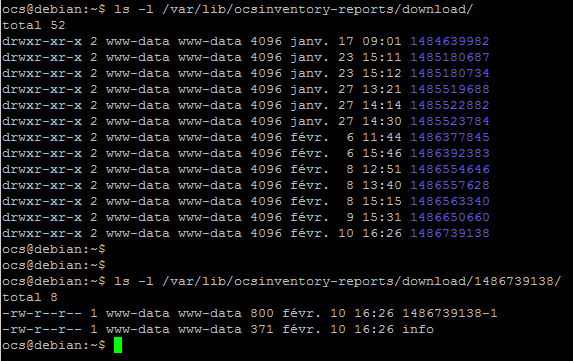
\includegraphics[scale=0.7]{Script/Deploiement5.PNG}
\caption{Résultat coté serveur}
\end{figure}
\newpage
\subsubsection{Activation}

Après avoir eu la confirmation de la création du paquet, il reste à l'activer pour pouvoir le déployer sur les Postes. Et pour ce faire, il faut faire la même opération de tout à l'heure mais cette fois, il faut cliquer sur \textbf{"Activate"}

\begin{figure}[hbtp]
\centering
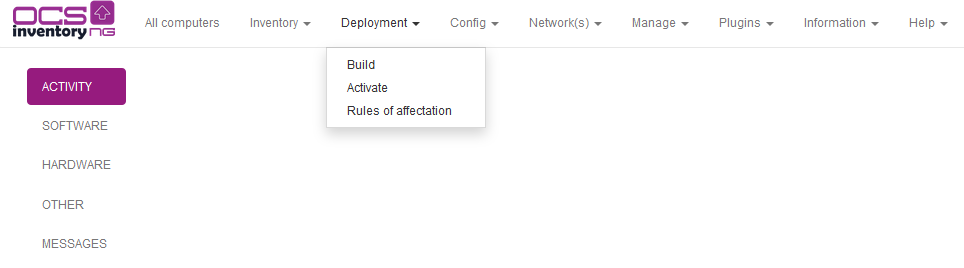
\includegraphics[scale=0.7]{Script/Deploiement1.PNG}
\caption{Accès Activation Paquet}
\end{figure}

Après avoir cliqué dessus, la page \textbf{"Package Activation"} s'ouvre en y montrant la liste des paquets disponibles pour le déploiement.

\begin{figure}[hbtp]
\centering
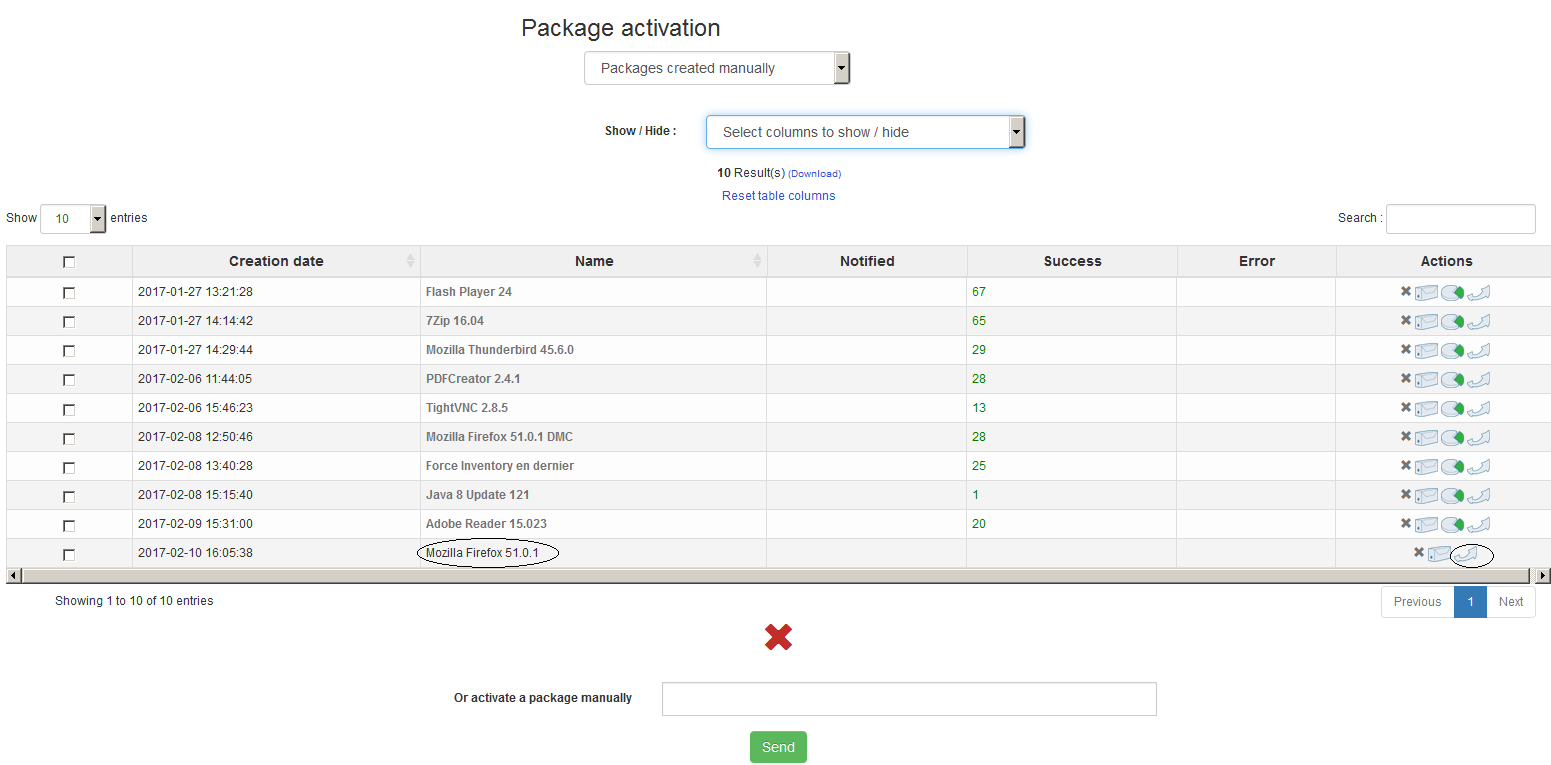
\includegraphics[scale=0.4]{Script/Activation2.PNG}
\caption{Accès Activation Paquet}
\end{figure}
 
Par rapport aux autres paquets déjà déployés, celui qu'on à crée est affiché différemment, \textbf{il apparait en "Noir"} alors que \textbf{les autres apparaissent en "Gris"} car ils ont été activés et pas le nôtre. Pour ce faire, il faut sur la "Flèche en double sens" à droite de l'écran. Suite à ça, il demande confirmation pour l'activation et ensuite notre \textbf{paquet devient "Grisé"} comme les autres.
\newpage
\subsubsection{Déploiement sur les postes}
Après que les paquets soit créés et activés, il reste à les déployer sur les postes, pour cela, il suffit de retourner sur la liste d'ordinateur qui se trouve dans \textbf{"All Computers"} et à choisir le poste en cliquant sur le nom du poste...
\begin{figure}[hbtp]
\centering
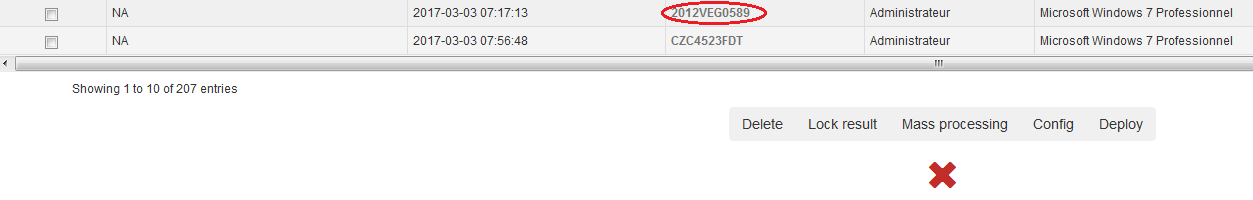
\includegraphics[scale=0.5]{Script/Act_Deploy1.PNG}
\caption{Choix du poste}
\end{figure}

... et en vérifiant les logiciels déjà existants pour pas installer un logiciel inutile sur le poste en naviguant sur la fiche du poste puis dans l'onglet \textbf{"Softwares"} ou sinon pour un nouveau poste, il faut aller directement sur \textbf{"Déployment"}.
\begin{figure}[hbtp]
\centering
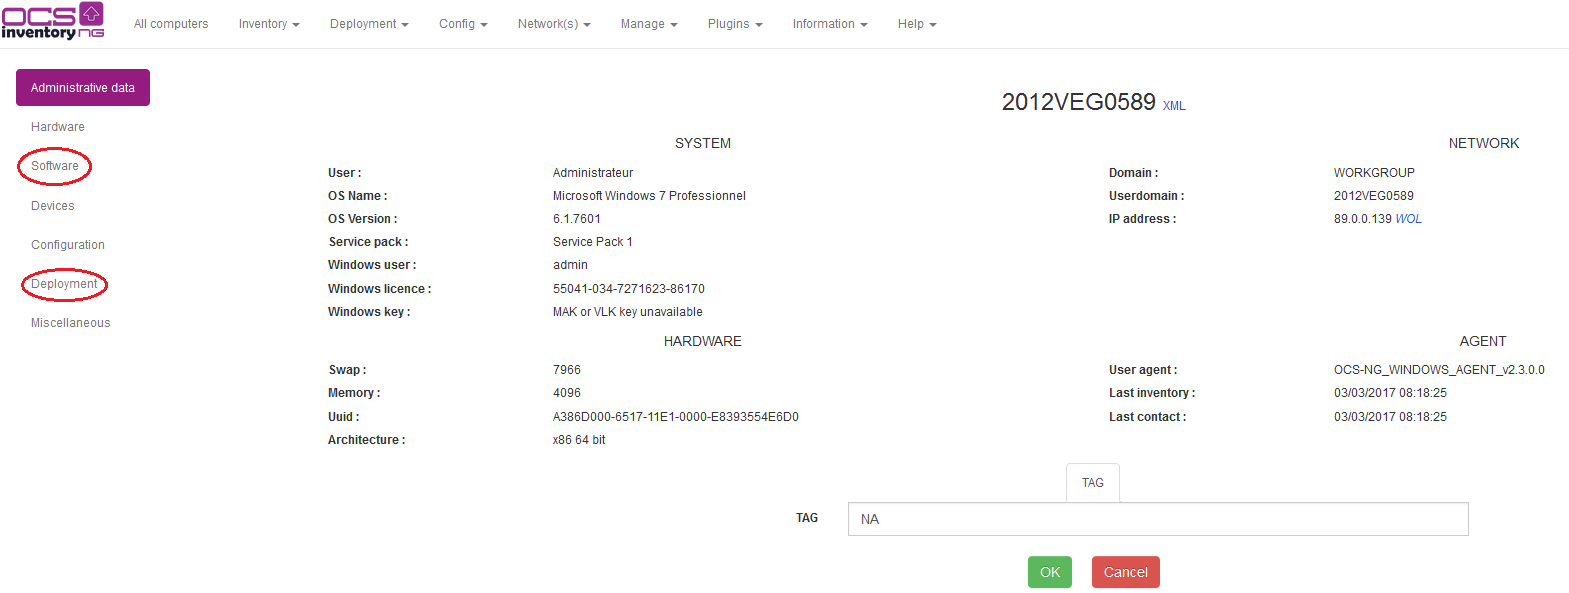
\includegraphics[scale=0.41]{Script/Act_Deploy2.PNG}
\end{figure}
\\
Suite à ça, dans le menu \textbf{"Déployment"} il faut ajouter le paquet crée précédemment pour le mettre en file d'attente et qui sera déployer lors du prochain inventaire du poste. Il suffit de cliquer sur le bouton \textbf{"Add Package"} puis choisir ou non les options avancées du déploiement.
\begin{figure}[hbtp]
\centering
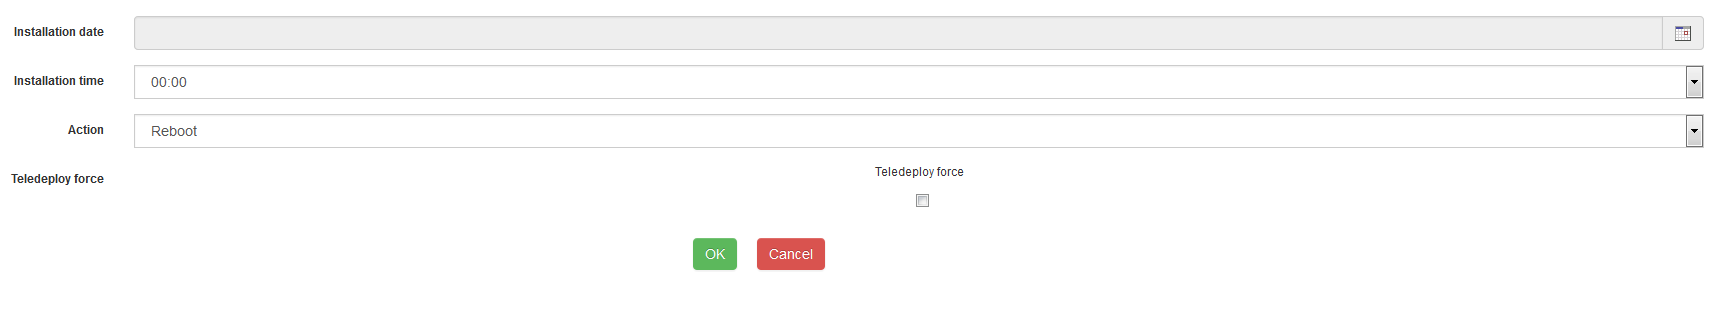
\includegraphics[scale=0.4]{Script/Act_Deploy4.PNG}
\caption{Options avancées}
\end{figure}

C'est-à-dire que si on choisit \textbf{"YES"} et qu'après on choisit le paquet voulu, il demande la \textbf{date et l'heure d'installatio}n et en fin de déploiement, si on veut \textbf{redémarrer ou éteindre} le poste mais dans notre cas, il faut \textbf{SURTOUT PAS} le faire. Quand le paquet à été choisi, il reste à retourner sur la page de déploiement du poste et voir qu'il y a le paquet qui est en attente. Le paquet sera déployer au prochain inventaire ou on peut le forcer en utilisant \textbf{PSEXEC (en mode administrateur)}
\newpage
\section{Annexes}
\subsection{Scripts}
\textbf{Script avec MSIEXEC (pour les packages .msi).}
\begin{figure}[hbtp]
\centering
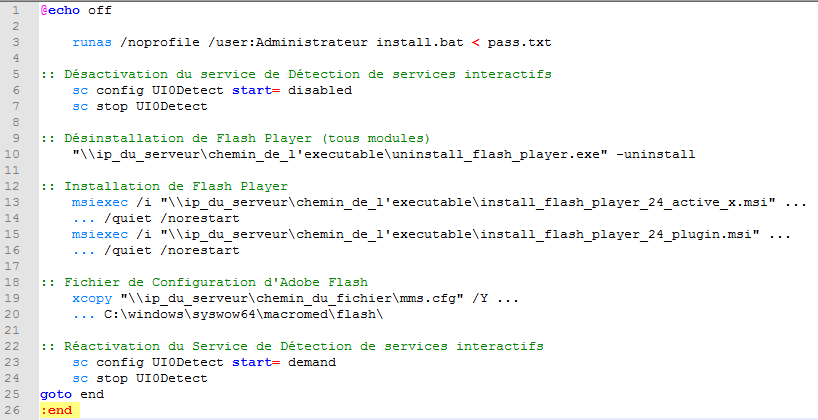
\includegraphics[scale=0.9]{Script/Flash.PNG}
\end{figure}

Le script est à peu près le même que pour celui de Mozilla Firefox crée précédemment sauf que cette fois, il s'agit d'un package .MSI.\\
En détail sur les lignes de désinstallation et d'installation : (Cf.Annexes) \\
\begin{itemize}
\item Ligne 10 : L'exécutable .exe permet de supprimer TOUTES les versions d'Adobe Flash Player présente sur 			l'ordinateur de manière silencieuse vu qu'on lui ajoute le paramètre "-uninstall" \\

\item Ligne 12 - 16 : Le package .MSI démarrera en mode silencieux et sans redémarrer comme indiquer avec les paramètres "/quiet" et "/norestart"
\end{itemize}
\newpage
\textbf{Script PowerShell pour changer les raccourcis Internet des Postes Clients}
\begin{figure}[hbtp]
\centering
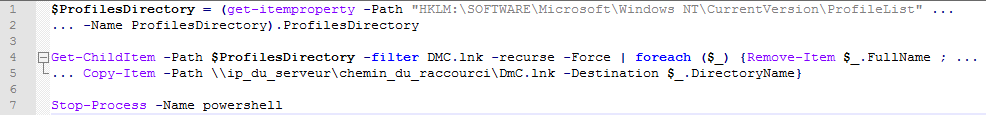
\includegraphics[scale=0.6]{Script/Powershell.PNG}
\end{figure}
\textbf{Commentaires :}\\
\begin{itemize}
\item \textbf{Variable \$ProfileDirectory :} Récupère à partir du registre, les répertoires Utilisateurs existants dans le Disque Local C: 
\item \textbf{Commande Get-ChildItem :} Depuis la variable \$ProfilesDirectory, le script va filtré dans tout les dossiers utilisateur l'icône "DMC.lnk" en la supprimant (si trouvé) et en copiant depuis le serveur la nouvelle icône fonctionnelle 
\end{itemize}

\subsection{Définitions}
\textbf{Microsoft Hyper-V :} Virtualisation de machines en ayant le service d'installer sur un Windows 8.x minimum, fonctionne à peu près comme VirtualBox
\\ \\
\textbf{PSEXEC :} PsExec est un outil en ligne de commande. Il permet d’exécuter à distance des commandes, des programmes, des batch, comme si vous étiez connecté sur le postes distant.
\\ \\
\textbf{RUNAS :} La commande RUNAS permet à un utilisateur d'exécuter des outils et des programmes spécifiques avec des autorisations différentes de celles attribuées à l'ouverture de session; par exemple, si vous désirez exécuter un programme nécessitant des droits d'Administrateur alors que vous n'êtes pas connecté en tant que tel.
\\ \\
\textbf{Commande SC :} L'utilitaire de contrôle des services SC est un puissant outil en ligne de commande permettant de gérer les services Windows. Cet outil permet également d'arrêter et de démarrer rapidement les services afin de résoudre les problèmes.
\\ \\
\textbf{U10Detect :} Active la notification des entrées utilisateur pour les services interactifs, qui active l'accès aux boîtes de dialogue créées par les services interactifs lorsqu'elles apparaissent.
\\ \\
\textbf{MSIEXEC :} La commande \textbf{msiexec} utilise des paramètres pour donner à MSI une partie ou l'ensemble des informations pouvant être spécifiées au sein d'une installation interactive. Cela signifie qu'un utilisateur peut créer une configuration d'installation automatique ou semi-automatique réutilisable. Les paramètres peuvent être fournis via la ligne de commande, un fichier de conversion, un fichier de réponse ou une combinaison des trois
\newpage

\section{Références}
\begin{itemize}
\item \textbf{Adobe :} \url {http://www.adobe.com/fr/} 
\item \textbf{Java :} \url {https://www.java.com/fr/}
\item \textbf{Mozilla :} \url {https://www.mozilla.org/fr/}
\item \textbf{PDFCreator :} \url {http://www.pdfforge.org/pdfcreator}
\item \textbf{Debian 8.x :} \url {https://www.debian.org/index.fr.html} 
\item \textbf{OCS Inventory NG :} \url {www.OCSinventory-ng.org/fr/} et aussi : \url {https://github.com/OCSInventory-NG}
\item \textbf{WAPT :} \url {https://dev.tranquil.it/wiki/WAPT_-_apt-get_pour_Windows}
\item \textbf{WSUS Package Publisher :} \url {https://wsuspackagepublisher.codeplex.com/}
\item \textbf{Local Update Publisher :} \url {http://localupdatepubl.sourceforge.net/fr/index.html}
\item \textbf{Wiki d'OCS Inventory :} \url{http://wiki.OCSinventory-ng.org/index.php?title=Documentation:Server/fr}
\item \textbf{OCS Inventory NG Agent Deployment Tool :} \url {http://wiki.ocsinventory-ng.org/index.php?title=Documentation:DeployTool/fr}
\item \textbf{PSEXEC :} \url {https://technet.microsoft.com/fr-fr/sysinternals}
\end{itemize}
\end{document}
